

\chapter{ESP32-CAM}\label{ESP32description}



\begin{figure}
    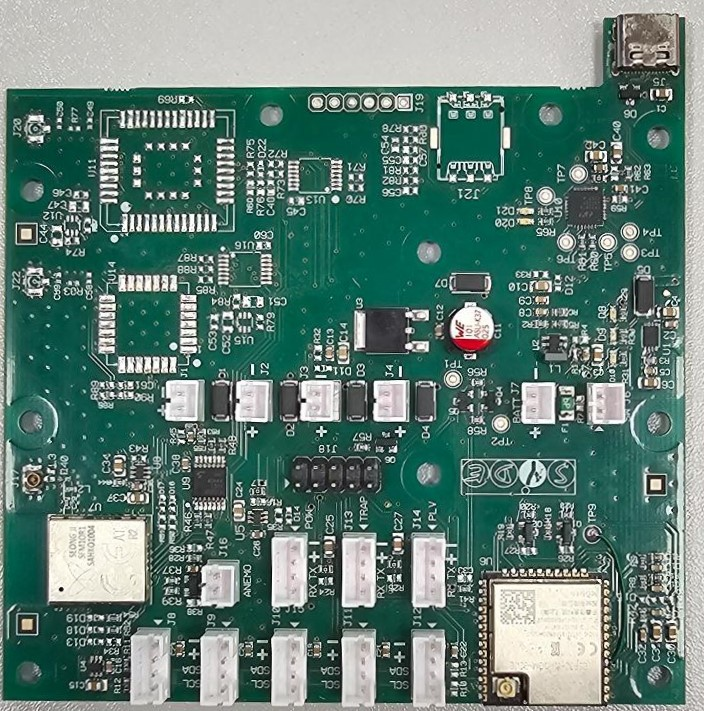
\includegraphics[width=\textwidth]{Syde/SydeESS}
    \caption{Syde’s ESP32 Eco Sensor System}
\end{figure}

\section{ESP32-CAM}\label{ESP32description}

The \ac{esp32cam} is a low-cost full-featured microcontroller with an \ac{esp32}-S development board along with an onboard camera module and micro-\ac{sd} card port. In addition, this board has integrated \ac{wifi} and \ac{ble}, which allows it to transfer data wirelessly when required.

\medskip

The \ac{esp32cam} is a versatile development board that combines an \ac{esp32}-S chip, a microcontroller with integrated \ac{wifi} and Bluetooth capability, with a camera module, making it a compact solution for various \ac{iot} and \ac{diy} projects. This board integrates a 2 \ac{mp} camera and supports the Arduino \ac{ide}, enabling easy programming and interfacing with other devices. 

\medskip

The \ac{esp32cam} with its onboard capabilities and connectivity options, the \ac{esp32cam} finds applications in surveillance systems, smart home automation, remote monitoring, and other projects requiring both wireless communication and visual data acquisition. Its affordability, compact size, and extensive capabilities make it a popular choice among hobbyists, developers, and enthusiasts exploring the realms of \ac{iot} and embedded systems.

\medskip

\ac{esp32cam} is readily available in different \ac{hw} Distributors online with costs ranging from around 10 Euros to 20 Euros, depending on other additional gadgets included, such as Development Board, Serial Converter, and others required for larger scale projects.

\medskip

The small form factor, availability and economic feasibility of the \ac{esp32} make it a perfect solution for various IoT applications such as wireless monitoring, quick response code identification, image tracking, image recognition, smart home devices, industrial wireless control and other applications.

\medskip

The \ac{esp32cam} is employed in this project due to its integrated camera and processing capabilities. Its onboard camera, combined with the computational power of the \ac{esp32} microcontroller, allows for real-time image capture and processing. With the appropriate programming, libraries, and algorithms which have been discussed in the previous chapters, the \ac{esp32cam} can efficiently decode and interpret barcodes, making it an ideal choice for applications requiring barcode scanning.

\section{Components in ESP32CAM Development Board}



\begin{figure}[!ht]
    \centering
    \resizebox{1\textwidth}{!}{%
        \begin{tikzpicture}
            \tikzstyle{every node}=[font=\large]
            
            \draw  (7.5,9.75) rectangle (14.75,-0.25); %big rectangle
            \draw[fill=silver] (9.5,9.75) rectangle (13,6.75); %SD Card Slot
            \draw[fill=black]  (10.5,8.5) rectangle (12.25,6.75); %small SD
            \draw[fill=silver] (9.5,2.75) rectangle (13,1.5);  %Camera Connection
            \draw[fill=yellow]  (13.5,2) rectangle  (14.5,1); %Flash Lamp
            
            % Dashed circles
            \foreach \y in {8.25, 7.5, 6.75, 6, 5.25, 4.5, 3.75, 9.25, 8.5, 7.75, 7, 6.25, 5.5, 4.75, 4} {
                \draw[dashed, orange] (8,\y) circle (0.25cm);
                \draw[dashed, orange] (14,\y) circle (0.25cm);
            }
            
            % Arrows and labels
            \draw [](10.75,11.5) -- (10.75,9.75);
            \draw [](6.5,9.25) -- (7.5,9.25);
            \draw [](6.75,4) -- (7.5,4);
            \draw [](6.5,9.25) -- (6.5,4);
            \draw [](6.5,4) -- (6.75,4);
            \draw [](5.75,6.75) -- (6.5,6.75);
            \draw [](14.25,8.25) -- (15.25,8.25);
            \draw [](14.25,5.25) -- (15.25,5.25);
            \draw [](13.75,3.25) -- (15.25,3.25);
            \draw [](14.5,1.5) -- (15.5,1.5);
            \draw [](6.25,2) -- (9.25,2);
            
            % Text nodes
            \node at (10.5,12) {SD Card Slot};
            \node at (16.25,8.25) {TF Card Holder};
            \node at (16.75,5.25) {Voltage Regulator Chip};
            \node at (16.5,3.25) {FPC Connector};
            \node at (16.5,1.5) {Flash Lamp};
            \node at (4.5,6.75) {Pin Coatings};
            \node at (4.5,2) {Camera Connection};
            \node at (10.75,0.25) {\texttt{ESP32-CAM}};
            
        \end{tikzpicture}%
    }
    \caption{ESP32-CAM Components}
    \label{fig:esp32_components}
    
    
\end{figure}



The \ac{esp32cam} development board has the following nine components as explained and shown in Figure \ref{fig:esp32_components} and \ref{fig:esp32s_components}: 

\begin{enumerate}
    \item \textbf{\ac{esp32}-S Chip}: This is the main module which houses dual core high-performance 32-bit LX6 \ac{cpu}s. It computes all the processing and functioning. This supports Wireless Fidelity (Wi-Fi) and Bluetooth 4.2
    
    \item \textbf{IPEX block output}: The IPEX acts a connector to Global System for Mobile communication (GSM) antennas to transmit signals.
    
    \item \textbf{Tantalum capacitor}: Tantalum capacitor is used to provide power supply filtering for fine signal quality.
    
    \item \textbf{Reset button}: The reset button restarts the code that is executed on the module when pressed.
    
    \item \textbf{Voltage regulator chip}: The voltage regulator chip is used to regulate the voltage to 3.3 volts. This ensures that the module maintains a constant output voltage despite the fluctuations in the input power supply.
    
    \item \textbf{PSRAM}: This module is the Pseudo-Random-Access Memory. It consists of about 4MB memory. This enables quick processing of the instruction provided to it and assists the \ac{esp32} camera run smoothly.
    
    \item \textbf{\ac{tfcard} Holder}: \ac{tfcard} Holder houses the Micro-\ac{sd} card which stores the data in ESP32. The transmission of data between card and the \ac{esp32}-S chip takes place through the Serial Peripheral Interface.
    
    \item \textbf{FPC connector}: The Flexible Printed Circuit (FPC) connectors is used to mount the camera. The fine pitch of the FPC ensures the reliability of signal.
    
    \item \textbf{Flash Light}: The flash light module produces electric pulses which illuminates the area acts as a flash for the camera in order to take clear pictures.
\end{enumerate}


\begin{figure}  
    \begin{center}
        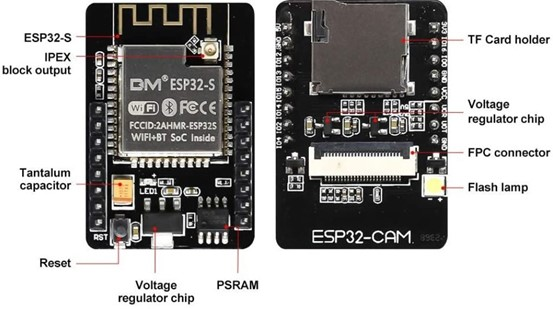
\includegraphics[width=12cm]{ESP32/ESP32components}
        \caption{Components in ESP32-CAM} 
        \label{fig:Components in ESP32 Cam}
        \footnotesize \textbf{Reference:} \cite{MicrocontrollersLab:2021}
    \end{center}
\end{figure}


\begin{figure}[!ht]
    \centering
    \resizebox{0.8\textwidth}{!}{%
        \begin{tikzpicture}
            \tikzstyle{every node}=[font=\large]
            
            % Component rectangles
            \draw  (5.25,12.5) rectangle (14,1);
            \draw[fill=silver] (7.25,10.25) rectangle (12.5,5.25);
            \draw[fill=black] (7.25,11) rectangle (7.75,12);
            \draw[fill=black] (6.5,10.25) rectangle (7.25,8.75);
            \draw[fill=black] (7.5,2.25) rectangle (9,1.5);
            \draw[fill=black] (12.75,2.25) rectangle (13.75,1.25);
            \draw[fill=black] (6.25,2.25) rectangle (6.75,1.25);
            \draw[fill=black] (4.25,4.5) rectangle (5.25,4.5);
            \draw[fill=black] (6.5,1) rectangle (6.5,-0.25);
            \draw[fill=black] (8.25,1.5) rectangle (8.25,-0.25);
            \draw[fill=black] (13.25,1.25) rectangle (13.25,-0.25);
            
            % Dashed circles
            \foreach \y in {1.75, 2.75, 4, 5, 6, 7, 8.25, 9.5} {
                \draw[dashed, orange] (13.25,\y) circle (0.25cm);
                \draw[dashed, orange] (5.75,\y) circle (0.25cm);
            }
            
            % Arrows
            \draw (7.75,12) -- (7.75,11.5) -- (8,11.5) -- (8.25,11.5) -- (8.25,12) -- (8.75,12) -- (8.75,11.5) -- (9.25,11.5) -- (9.25,12) -- (10.5,12) -- (10.5,10.75);
            \draw (10.5,12) -- (11,12) -- (11,10.75);
            \draw (13,12.5) -- (13,10.75);
            \draw (4.25,9.75) -- (6.5,9.75);
            \draw (4.25,11.25) -- (7.25,11.25);
            \draw (8.25,-0.25) -- (8.25,-1);
            
            % Text nodes
            \node at (3,11.25) {ESP32-S};
            \node at (2.75,9.75) {IPEX Block Output};
            \node at (2.25,4.5) {Tantalum Capacitor};
            \node at (13.25,-0.5) {PSRAM};
            \node at (8.25,-1.25) {Voltage Regulator Chip};
            \node at (6.5,-0.5) {Reset};
        \end{tikzpicture}%
    }
    \caption{ESP32-S Components}
    \label{fig:esp32s_components}
    
    
    
\end{figure}

%%%%%%%%%%%%%%%%%%%%%%%%%%%%%%%

\section{ESP32-CAM Microcontroller Features}\label{ESP32specifications}

The \ac{esp32cam} microcontroller has the ESP32-S microprocessor module. The following are the data processing and \ac{hw} capabilities.

\begin{itemize}
    \item Has 802.11b/g/n Wi-Fi SoC Module with a speed of 2.4 GHz
    \item Has Bluetooth 4.2 with \ac{ble}
    \item Has a Low-power dual-core 32-bit \ac{cpu} for application processing
    \item Clock speed up to 160 MHz
    \item Has a summary computing power goes up to 600 DMIPS
    \item Has a Built-in 520 KB SRAM plus 4 MB PSRAM
    \item Supports \ac{uart}, SPI, \ac{i2c}, and \ac{pwm} interfaces
    \item Supports Wi-Fi Image Upload
    \item Supports multiple sleep modes
    \item Firmware Over the Air (FOTA) upgrades are possible
    \item 9 \ac{gpio} ports are available
    \item Has a Built-in Flash \ac{led}
    \item Support \ac{tfcard}
    \item Has an onboard \ac{pcb} antenna
    \item Has embedded Free \ac{rtos} and lightweight IP
\end{itemize}


\section{ESP32-S Microprocessor Specification}

The following are the specification of the \ac{esp32cam}:

\begin{itemize}
    \item SPI Flash: default 32Mbit
    \item RAM: built-in 520 KB + external 4MPSRAM
    \item Dimension: 27*40.5*4.5(±0.2)mm1.06*1.59*0.18”
    \item Bluetooth: Bluetooth 4.2 BR/EDR and \ac{ble} standards
    \item Wi-Fi: 802.11b/g/n/e/i
    \item Support Interface: \ac{uart}, SPI, \ac{i2c}, \ac{pwm}
    \item Support TF card: maximum support 4G
    \item IO port: 9
    \item Serial Port Baud-rate: Default 115200 bps
    \item Image Output Format: JPEG( \ac{ov2640} support only ), BMP, GRAYSCALE
    \item Spectrum Range: 2412 ~2484MHz
    \item Antenna: onboard \ac{pcb} antenna, gain 2dBi
    \item Transmit Power: 802.11b: 17±2 dBm (@11Mbps);
    802.11g: 14±2 dBm (@54Mbps);                              802.11n: 13±2 dBm (@MCS7)
    \item Receiving Sensitivity: CCK, 1 Mbps: -90dBm;
    CCK, 11 Mbps: -85dBm; 
    6 Mbps (1/2 BPSK): -88dBm;
    54 Mbps (3/4 64-QAM): -70dBm;
    MCS7 (65 Mbps, 72.2 Mbps): -67dBm
    \item Power consumption: Flash Off: 180mA@5V
    Flash On and maximum brightness:310mA@5V             Deep-sleep: 6mA@5V                                    Moderm-sleep:20mA@5V                                  Light-sleep: 6.7mA@5V
    \item Security: WPA/WPA2/WPA2-Enterprise/WPS
    \item Power supply range: 5V
    \item Operating temperature: -20 °C ~ 85 °C
    \item Storage environment: -40 °C ~ 90 °C, < 90%RH
    \item Weight: 10g
\end{itemize}

\section{How to Program ESP32-CAM}

Programming an ESP32-CAM for the project involves setting up the ESP32-CAM to capture images with its camera and integrating a barcode scanning module to decode the barcode data. Below are the steps to program the ESP32-CAM for this purpose:

\bigskip

\textbf{Components Needed:}

\begin{enumerate}
    \item ESP32-CAM module
    \item Barcode scanner module
    \item Stable power supply for ESP32-CAM
    \item Wires and connectors
\end{enumerate}

\textbf{Hardware Setup:}

\begin{itemize}
    \item \textbf{Power Supply:}
    \begin{itemize}
        \item Ensure that you have a stable 5V power source to power both the ESP32-CAM and the barcode scanner module. This can be achieved using a USB cable or an external power supply connected to the ESP32-CAM's power input pins.
        \item It's crucial to provide adequate power, as the ESP32-CAM and the barcode scanner might have varying power requirements. Insufficient power can lead to unstable behavior.
    \end{itemize}
    \item \textbf {Connections:}
    \begin{itemize}
        \item Identify the TX (Transmit) and RX (Receive) pins on both the ESP32-CAM and the barcode scanner module. These pins are used for serial communication between the devices.
        \item Use jumper wires to connect the TX pin of the barcode scanner module to the RX pin of the ESP32-CAM, and connect the RX pin of the barcode scanner module to the TX pin of the ESP32-CAM.
        \item Make sure to connect the ground (GND) pin of the barcode scanner module to the ground (GND) pin of the ESP32-CAM to establish a common ground.
        \item Refer to the datasheets or documentation of your specific barcode scanner module for pinouts and voltage levels to ensure correct connections.
    \end{itemize}
    \item \textbf {Physical Placement:}
    \begin{itemize}
        \item Position the components in a way that facilitates easy scanning of barcodes by the scanner. Ensure that the barcode scanner module has a clear line of sight to scan barcodes effectively.
    \end{itemize}
    \item \textbf {Double Check Connections:}
    \begin{itemize}
        \item Before powering up, double-check all the connections to ensure they are correctly wired. Miswiring could potentially damage the components or lead to malfunction.
    \end{itemize}
    \item \textbf {Testing:}
    \begin{itemize}
        \item Power up the setup and verify the connections by testing the barcode scanner's functionality. Use the Serial Monitor in the Arduino IDE to check if the ESP32-CAM receives data from the barcode scanner correctly.
    \end{itemize}
\end{itemize}

\textit{Notes:}
\begin{enumerate}
    \item Use the appropriate voltage levels for communication between the ESP32-CAM and the barcode scanner. Some barcode scanners operate at 5V logic levels, while the ESP32-CAM usually operates at 3.3V logic levels. Ensure proper level shifting if required.
    \item Consider using voltage dividers, level shifters, or logic level converters to interface between devices with different voltage requirements to prevent damage to the components.
    \item Always refer to the datasheets, technical documentation, or user manuals provided with your ESP32-CAM and barcode scanner module for specific wiring diagrams and precautions.
\end{enumerate}

\bigskip

The software setup is detailed in the further section \textit{Software}.

\bigskip

\section{Connection of the ESP32 to the PC}

Connecting the ESP32-CAM to a PC for a barcode reader project involves establishing a physical connection and communication between the ESP32-CAM module and the computer. Here are the reqirements and steps explained in detail:

\bigskip

\textbf{Requirements:}

\begin{enumerate}
    \item ESP32-CAM module
    \item USB cable 
    \item IDE installed on the PC
\end{enumerate}

\textbf{Steps to Connect ESP32-CAM to PC:}

\begin{itemize}
    \item \textbf{Prepare the ESP32-CAM:}
    \begin{itemize}
        \item Ensure the ESP32-CAM module is set up and ready for programming. This includes having the necessary libraries installed and the code written for your barcode reader project.
        \item Make sure the ESP32-CAM is powered either through a USB connection or an external power supply.
    \end{itemize}
    \item \textbf {Connect the ESP32-CAM to PC:}
    \begin{itemize}
        \item Use a USB cable (usually micro-USB) to establish a connection between the ESP32-CAM module and your PC. Connect one end of the USB cable to the USB port on your computer and the other end to the USB port on the ESP32-CAM module.
        \item Ensure that the USB cable is securely plugged into both the ESP32-CAM and your PC.
    \end{itemize}
    \item \textbf {Install Drivers:}
    \begin{itemize}
        \item In most cases, the ESP32-CAM should automatically be recognized by your computer when connected via USB. However, if a computer requires drivers for the ESP32-CAM, there might be a need of installation, mostly from the manufacturer`s website.
    \end{itemize}
    \item \textbf {Identify COM Port:}
    \begin{itemize}
        \item Open the IDE on the PC and go to `Port` from `Tools`. 
        \item A new COM port is listed when the ESP32-CAM is connected correctly. Note down the COM port number as you'll need it to upload code to the ESP32-CAM.
    \end{itemize}
    \bigskip
    \item \textbf {Upload Code to ESP32-CAM:}
    \begin{itemize}
        \item Ensure that you have selected the correct board and COM port in the IDE (Tools > Board and Tools > Port).
        \item Open your barcode reader project code.
        \item Click on the Upload button to compile and upload the code to the ESP32-CAM.
    \end{itemize}	
\end{itemize}

\textit{Notes:}
\begin{enumerate}
    \item Ensure the USB cable is of good quality and capable of data transfer.
    \item Sometimes, a faulty USB cable might cause connectivity issues. Try using a different USB cable if you encounter problems.
    \item Make sure the ESP32-CAM is in programming mode when uploading code.
    \item Follow safety precautions and handle the ESP32-CAM and the USB cable carefully to prevent damage.
\end{enumerate}

The details regarding to software for connection of the ESP32 to the PC is given in the further section \textit{Software}.

%%%%%%%%%%%%%%%%%%%%%%%%%%%%%%%
\section{ESP32-CAM Camera Module}

\begin{figure}[!ht]
    \centering
    \resizebox{1\textwidth}{!}{%
        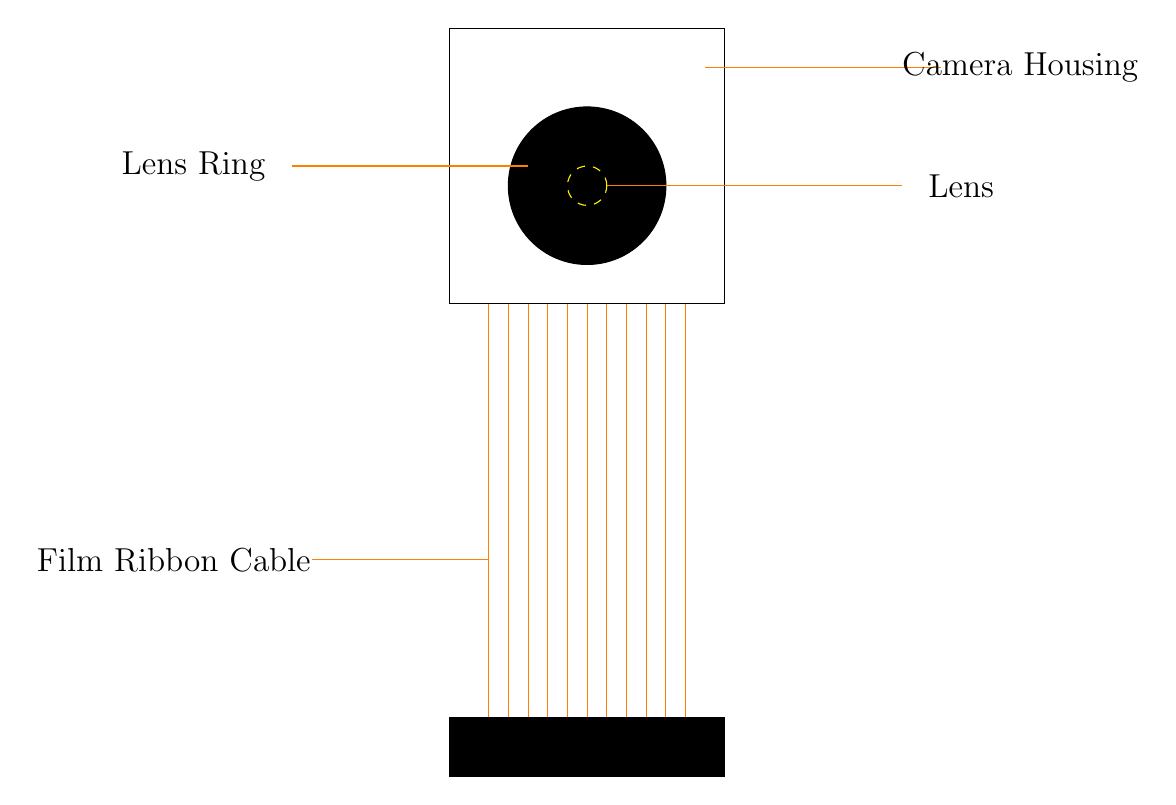
\begin{tikzpicture}
            \tikzstyle{every node}=[font=\large]
            \draw[black, fill=black]  (6.5,12.25) circle (1cm);
            \draw[black, dashed, yellow] (6.5,12.25) circle (0.25cm);
            \draw[black, orange] (5.25,10.75) -- (5.25,5.75);
            \draw[black, orange] (5.5,10.75) -- (5.5,5.75);
            \draw[black, orange] (5.75,10.75) -- (5.75,6);
            \draw[black, orange] (6,10.75) -- (6,5.5);
            \draw[black, orange] (6.25,10.75) -- (6.25,5.75);
            \draw[black, orange] (6.5,10.75) -- (6.5,5.75);
            \draw[black, orange] (6.75,10.75) -- (6.75,5.75);
            \draw[black, orange] (7,10.75) -- (7,5.75);
            \draw[black, orange] (7.25,10.75) -- (7.25,5.5);
            \draw[black, orange] (7.5,10.75) -- (7.5,5.75);
            \draw[black, orange] (7.75,10.75) -- (7.75,5.75);
            \draw  (4.75,14.25) rectangle (8.25,10.75);
            \draw[black, fill=black]  (4.75,5.5) rectangle (8.25,4.75);
            \draw[black, orange] (5.25,5.75) -- (5.25,5.5);
            \draw[black, orange] (5.5,5.75) -- (5.5,5.5);
            \draw[black, orange] (5.75,6) -- (5.75,5.5);
            \draw[black, orange] (6.25,6) -- (6.25,5.5);
            \draw[black, orange] (6.5,6) -- (6.5,5.5);
            \draw[black, orange] (6.75,6) -- (6.75,5.5);
            \draw[black, orange] (7,5.75) -- (7,5.5);
            \draw[black, orange] (7.5,6) -- (7.5,5.5);
            \draw[black, orange] (7.75,5.75) -- (7.75,5.5);
            \draw[black, orange] (6.75,12.25) -- (10.5,12.25);
            \draw[black, orange] (8,13.75) -- (11,13.75);
            \draw[black, orange] (3,7.5) -- (5.25,7.5);
            \draw[black, orange] (2.75,12.5) -- (5.75,12.5);
            \node [font=\large] at (1.5,12.5) {Lens Ring};
            \node [font=\large] at (1.25,7.5) {Film Ribbon Cable};
            \node [font=\large] at (11.25,12.25) {Lens};
            \node [font=\large] at (12,13.75) {Camera Housing};
        \end{tikzpicture}
    }%
    \caption{OV2640 Camera Module}
    \label{fig:ov2640_camera}
    
    
    %	\label{fig:my_label}
\end{figure}

\begin{figure}  
    \begin{center}
        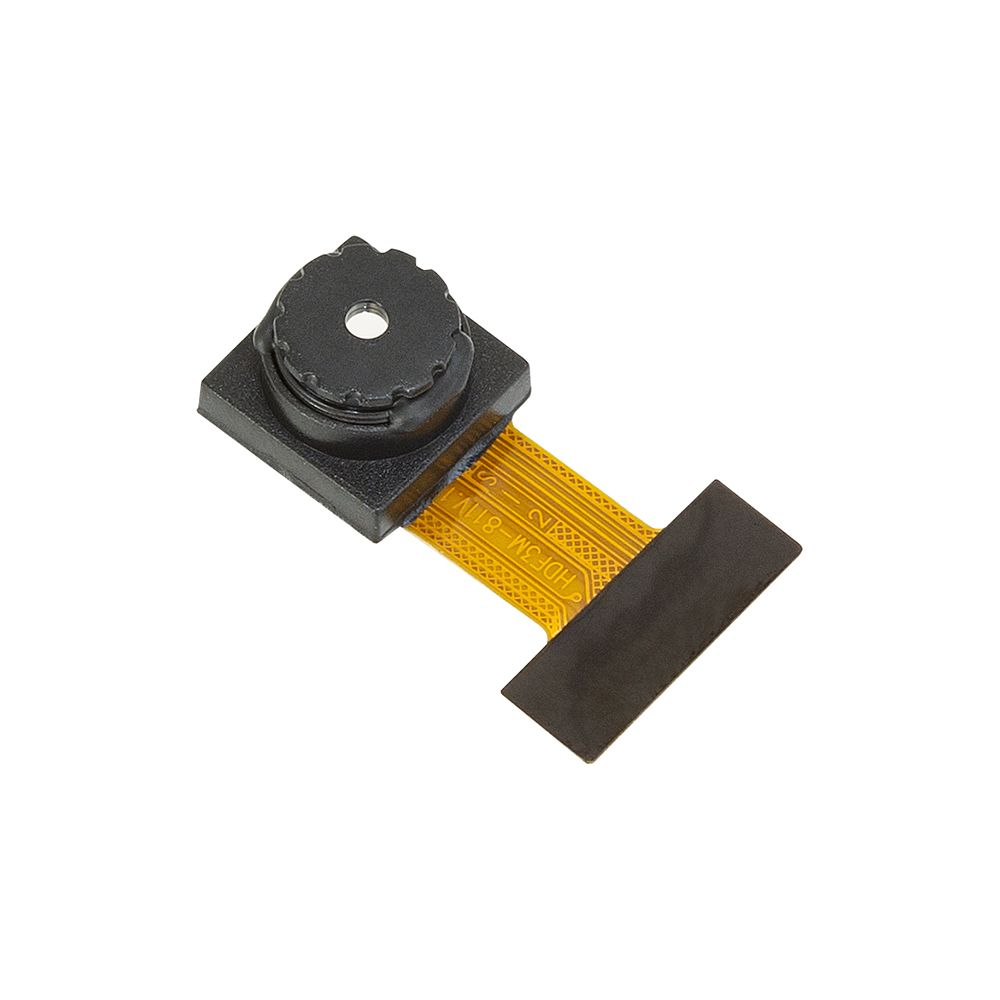
\includegraphics[width=12cm]{ESP32/OV2640}
        \caption{OV2640 Camera Module} 
        \label{fig:OV2640 Camera Module}
        \footnotesize \textbf{Reference:} \cite{}
    \end{center}                                   
\end{figure}

The \ac{esp32cam} uses the \ac{ov2640} camera module, which was the world’s first 1/4-inch 2 MP fully-integrated image sensor as shown in Figure \ref{fig:ov2640_camera}.The \ac{ov2640} image sensor has some notable features such as automatic exposure control (EC), automatic grain control (AGC), automatic white balance (AWB), automatic band filter (ABF), and automatic black-level calibration (ABLC). One of the most beneficial features of the \ac{ov2640} is its embedded compression engine which supports most common compression formats. The image sensor also allows the user to control the image quality controls such as sharpness (edge enhancement), colour saturation, white pixel canceling, noise reduction, variable frame rate and 50/60Hz luminance detection. \ac{ov2640} image sensor has high sensitivity for low-light operations and supports formats such as Raw RGB, RGB(RGB565/555), GRB22, YUV (422/420) and YCBCr (4:2:2) formats. 

\begin{center}
    \begin{table}[htbp]
        \begin{tabular}{|cc|l|}
            \hline
            \multicolumn{1}{|c|}{\textbf{Array Size}}                                                                              & \textbf{UXGA}                    & 1600 X 1200                               \\ \hline
            \multicolumn{1}{|c|}{\textbf{Power Supply}}                                                           & \textbf{Core}                    & 1.3VDC                                    \\ \cline{2-3} 
            \multicolumn{1}{|c|}{}                                                                                                 & \textbf{Analog}                  & $\sim$3.0VDC                              \\ \cline{2-3} 
            \multicolumn{1}{|c|}{}                                                                                                 & \textbf{I/O}                     & 1.7V to 3.3V                              \\ \hline
            \multicolumn{1}{|c|}{\textbf{Power Requirements}}                                                     & {\textbf{Active}} & 125 mW        \\ \cline{3-3} 
            \multicolumn{1}{|c|}{}                                                                                                 &                                  & 140 mW  \\ \cline{2-3} 
            \multicolumn{1}{|c|}{}                                                                                                 & \textbf{Standby}                 & 900 µA                                    \\ \hline
            \multicolumn{1}{|c|}{\textbf{Temperature Range}}                                                                       & \textbf{Stable Image}            & 0°C to 50°C                               \\ \hline
            \multicolumn{2}{|c|}{\textbf{Output Formats (8-bit)}}                                                                                    & • YUV(422/420)/YCbCr422                   \\ \cline{3-3} 
            \multicolumn{2}{|c|}{}                                                                                                                                    & • RGB565/555                              \\ \cline{3-3} 
            \multicolumn{2}{|c|}{}                                                                                                                                    & • 8-bit compressed data                   \\ \cline{3-3} 
            \multicolumn{2}{|c|}{}                                                                                                                                    & • 8-/10-bit Raw RGB data                  \\ \hline
            \multicolumn{1}{|c|}{\textbf{Lens Size}}                                                                               & \textbf{}                        & 1/4"                                      \\ \hline
            \multicolumn{1}{|c|}{\textbf{Chief Ray Angle}}                                                                         & \textbf{}                        & 25° non-linear                            \\ \hline
            \multicolumn{1}{|c|}{\textbf{\begin{tabular}[c]{@{}c@{}}Maximum Image \\ Transfer Rate\end{tabular}}} & \textbf{UXGA/SXGA}               & 15 fps                                    \\ \cline{2-3} 
            \multicolumn{1}{|c|}{}                                                                                                 & \textbf{SVGA}                    & 30 fps                                    \\ \cline{2-3} 
            \multicolumn{1}{|c|}{}                                                                                                 & \textbf{CIF}                     & 60 fps                                    \\ \hline
            \multicolumn{2}{|r|}{\textbf{Sensitivity}}                                                                                                                & 0.6 V/Lux-sec                             \\ \hline
            \multicolumn{2}{|r|}{\textbf{S/N Ratio}}                                                                                                                  & 40 dB                                     \\ \hline
            \multicolumn{2}{|r|}{\textbf{Dynamic Range}}                                                                                                              & 50 dB                                     \\ \hline
            \multicolumn{2}{|r|}{\textbf{Scan Mode}}                                                                                                                  & Progressive                               \\ \hline
            \multicolumn{2}{|r|}{\textbf{Maximum Exposure Interval}}                                                                                                  & 1247 x tROW                               \\ \hline
            \multicolumn{2}{|r|}{\textbf{Gamma Correction}}                                                                                                           & Programmable                              \\ \hline
            \multicolumn{2}{|r|}{\textbf{Pixel Size}}                                                                                                                 & 2.2 µm x 2.2 µm                           \\ \hline
            \multicolumn{2}{|r|}{\textbf{Dark Current}}                                                                                                               & 15 mV/s at 60°C                           \\ \hline
            \multicolumn{2}{|r|}{\textbf{Well Capacity}}                                                                                                              & 12 Ke                                     \\ \hline
            \multicolumn{2}{|r|}{\textbf{Fixed Pattern Noise}}                                                                                                        & \textless{}1\% of VPEAK-TO-PEAK           \\ \hline
            \multicolumn{2}{|r|}{\textbf{Image Area}}                                                                                                                 & 3590 µm x 2684 µm                         \\ \hline
            \multicolumn{2}{|r|}{\textbf{Package Dimensions}}                                                                                                         & 5725 µm x 6285 µm                         \\ \hline
        \end{tabular}
        
        \caption{OV2640 Camera Module Specification}
        \begin{center}
            \footnotesize \textbf{Reference:} 
        \end{center}
        
    \end{table}
\end{center}

%%%%%%%%%%%%%%%%%%%%%%%%%%%%%%%

\section{Interfaces}
In the context of the \ac{esp32} microcontroller, interfaces refer to the different communication and connectivity options that the \ac{esp32} offers to interact with other devices or systems. The \ac{esp32} is a versatile microcontroller that provides various interfaces to facilitate communication with peripherals, sensors, networks, and other devices. Some of the common interfaces available on the \ac{esp32} include:

\medskip

\begin{itemize}
    \item \textbf{\ac{gpio}:}The \ac{esp32} has a multitude of \ac{gpio} pins that can be configured as digital inputs or outputs. These pins can be used to interface with the barcode scanner module or other external devices like \ac{led}s, buttons, etc. For the project, \ac{esp32cam} is used for scanning.
    \item \textbf{\ac{uart} (Universal Asynchronous Receiver-Transmitter):} The \ac{esp32} has multiple \ac{uart} interfaces that allow serial communication. This interface is commonly used to communicate with barcode scanners that utilize \ac{uart} for data transmission. It enables the ESP32 to receive barcode data from the scanner.
    \item \textbf{SPI (Serial Peripheral Interface):} SPI is a synchronous serial communication interface commonly used for interfacing with sensors, displays, and other peripherals. The ESP32 provides multiple \ac{hw} SPI interfaces for high-speed communication.
    \item \textbf{\ac{i2c} (Inter-Integrated Circuit):} The \ac{esp32} supports \ac{i2c} communication, which is often used for interfacing with sensors and modules. Certain barcode scanners might use \ac{i2c} for communication, and the ESP32 can interface with such scanners using its \ac{i2c} pins. 
    \item \textbf{Pulse Width Modulation (\ac{pwm}):} By configuring \ac{pwm} channels on the \ac{esp32},  it is controlled the brightness of the reader's \ac{led}s, aiding in accurate barcode scanning. Additionally, \ac{pwm} can regulate motor speed in mechanisms responsible for moving the barcode reader's scanning components.
    \item \textbf{\ac{wifi} and Bluetooth Connectivity:} \ac{esp32} is known for its built-in \ac{wifi} and Bluetooth capabilities. These can be leveraged for sending barcode data wirelessly to other devices or services, enabling remote data logging, cloud connectivity, or communication with a mobile app. A mobile app is not in the scope of the project but it is considered as future improvements. The \ac{hw} of the project is connected by \ac{wifi}.
\end{itemize}

When developing a barcode reader project using the \ac{esp32}, understanding and utilizing these \ac{hw} interfaces effectively is crucial for interfacing with the barcode scanner module, processing the scanned data, and executing the necessary functionalities within the project.

\begin{figure}[!ht]
    \centering
    \resizebox{1.2\textwidth}{!}{%
        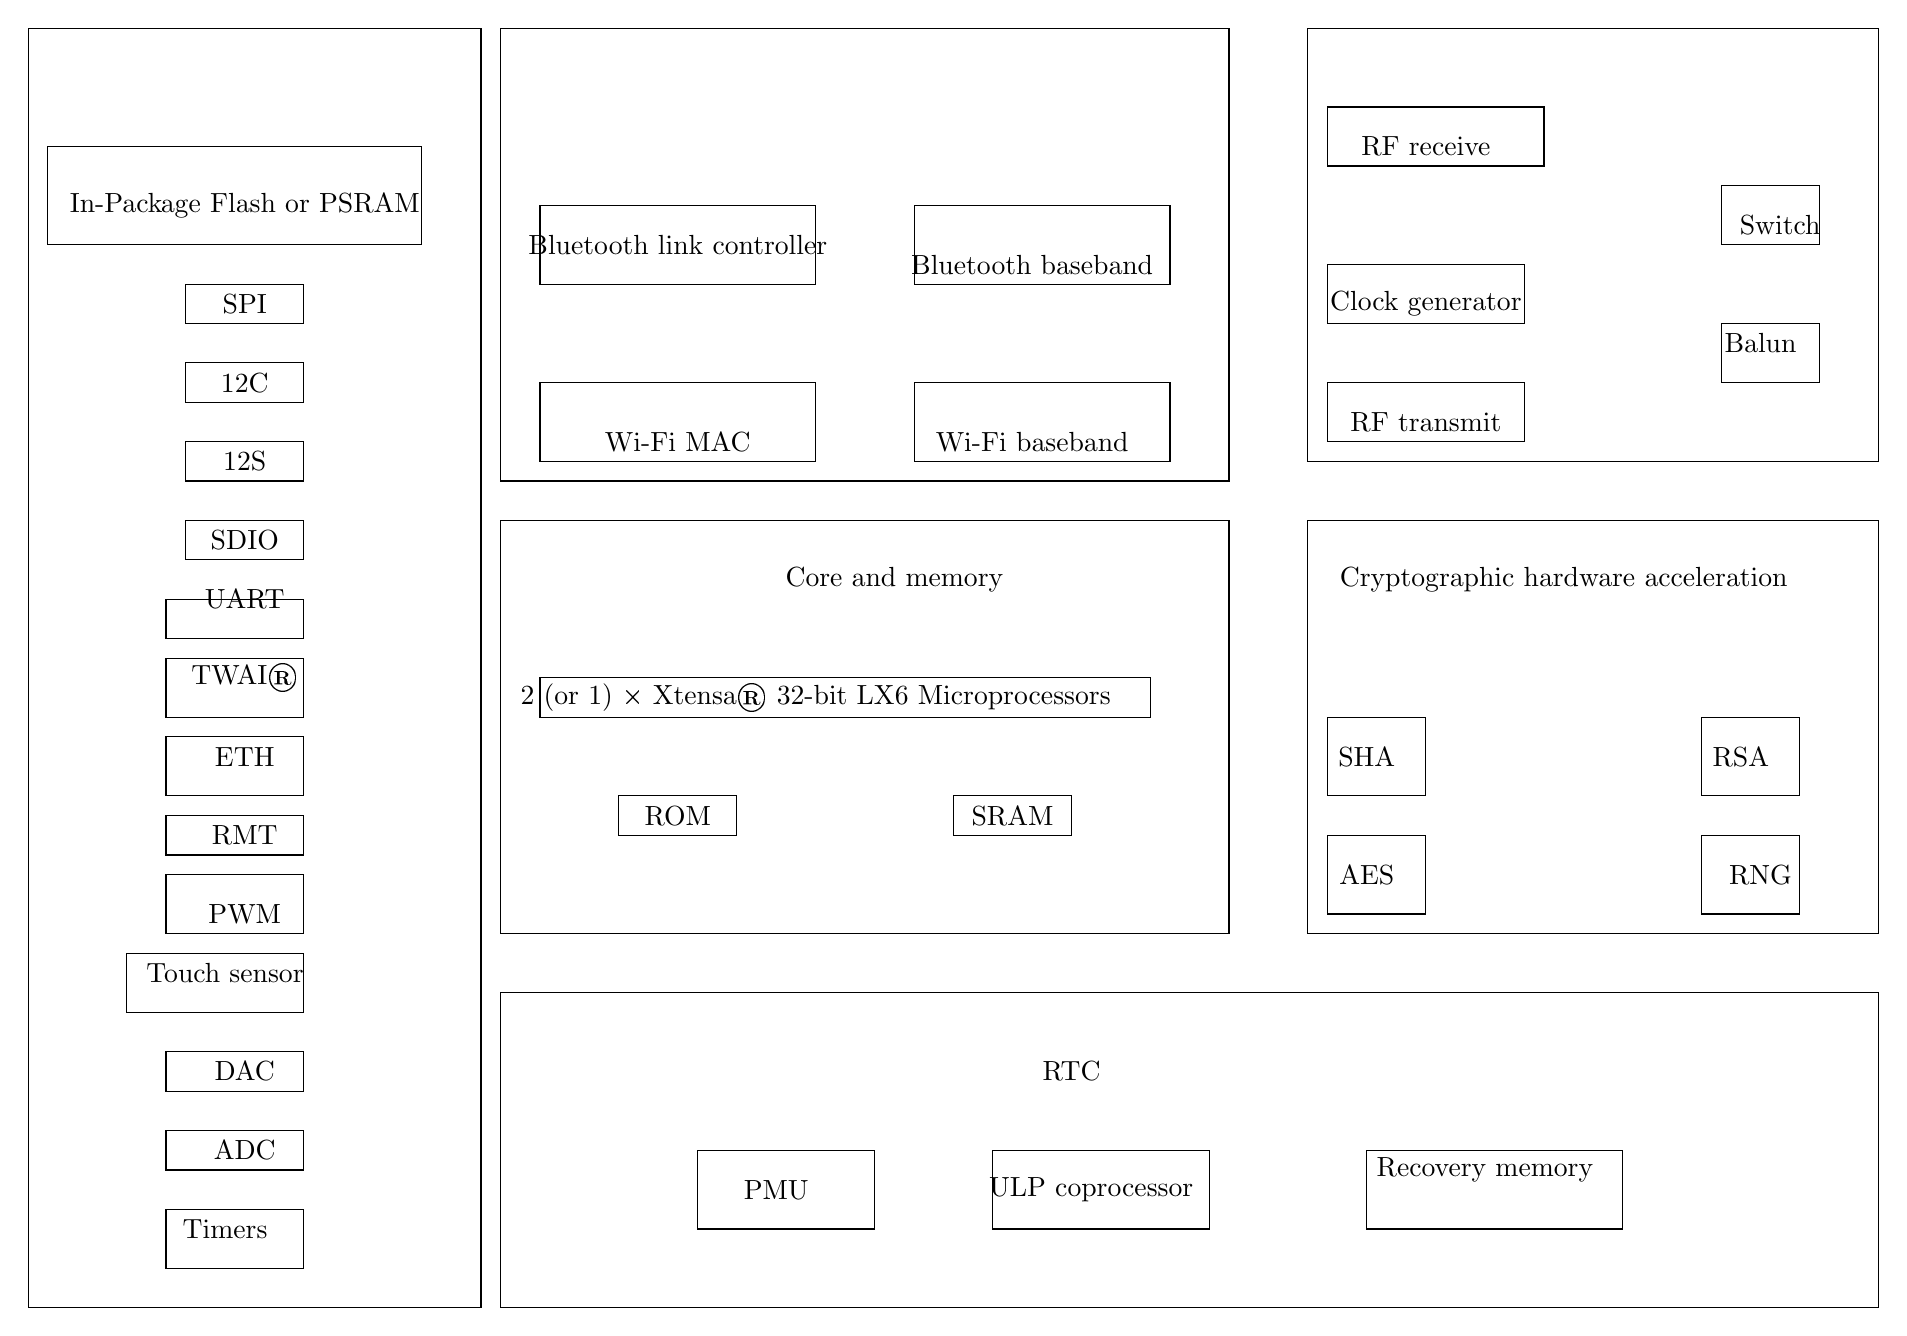
\begin{tikzpicture}
            \tikzstyle{every node}=[font=\normalsize]
            \node [font=\normalsize] at (0.5,13.75) {In-Package Flash or PSRAM};
            \node [font=\normalsize] at (0.5,12.5) {SPI};
            \node [font=\normalsize] at (0.5,11.5) {12C};
            \node [font=\normalsize] at (0.5,10.5) {12S};
            \node [font=\normalsize] at (0.5,9.5) {SDIO};
            \node [font=\normalsize] at (0.5,8.75) {UART};
            \node [font=\normalsize] at (0.5,7.75) {TWAI®};
            \node [font=\normalsize] at (0.5,6.75) {ETH};
            \node [font=\normalsize] at (0.5,5.75) {RMT};
            \node [font=\normalsize] at (0.5,4.75) {PWM};
            \node [font=\normalsize] at (0.25,4) {Touch sensor};
            \node [font=\normalsize] at (0.5,2.75) {DAC};
            \node [font=\normalsize] at (0.5,1.75) {ADC};
            \node [font=\normalsize] at (0.25,0.75) {Timers};
            \node [font=\normalsize] at (6,13.25) {Bluetooth link controller};
            \node [font=\normalsize] at (10.5,13) {Bluetooth baseband};
            \node [font=\normalsize] at (6,10.75) {Wi-Fi MAC};
            \node [font=\normalsize] at (10.5,10.75) {Wi-Fi baseband};
            \node [font=\normalsize] at (15.5,14.5) {RF receive};
            \node [font=\normalsize] at (15.5,12.5) {Clock generator};
            \node [font=\normalsize] at (15.5,11) {RF transmit};
            \node [font=\normalsize] at (20,13.5) {Switch};
            \node [font=\normalsize] at (19.75,12) {Balun};
            \node [font=\normalsize] at (8.75,9) {Core and memory};
            \node [font=\normalsize] at (7.75,7.5) {2 (or 1) × Xtensa® 32-bit LX6 Microprocessors};
            \node [font=\normalsize] at (6,6) {ROM};
            \node [font=\normalsize] at (10.25,6) {SRAM};
            \node [font=\normalsize] at (17.25,9) {Cryptographic hardware acceleration};
            \node [font=\normalsize] at (14.75,6.75) {SHA};
            \node [font=\normalsize] at (19.5,6.75) {RSA};
            \node [font=\normalsize] at (14.75,5.25) {AES};
            \node [font=\normalsize] at (19.75,5.25) {RNG};
            \node [font=\normalsize] at (11,2.75) {RTC};
            \node [font=\normalsize] at (7.25,1.25) {PMU};
            \node [font=\normalsize] at (11.25,1.25) {ULP coprocessor};
            \node [font=\normalsize] at (16.25,1.5) {Recovery memory};
            \draw  (-2,14.5) rectangle (2.75,13.25);
            \draw  (-0.25,12.75) rectangle (1.25,12.25);
            \draw  (-0.25,11.75) rectangle (1.25,11.25);
            \draw  (-0.25,10.75) rectangle (1.25,10.25);
            \draw  (-0.25,9.75) rectangle (1.25,9.25);
            \draw  (-0.5,8.75) rectangle (1.25,8.25);
            \draw  (-0.5,8) rectangle (1.25,7.25);
            \draw  (-0.5,7) rectangle (1.25,6.25);
            \draw  (-0.5,6) rectangle (1.25,5.5);
            \draw  (-0.5,5.25) rectangle (1.25,4.5);
            \draw  (-1,4.25) rectangle (1.25,3.5);
            \draw  (-0.5,3) rectangle (1.25,2.5);
            \draw  (-0.5,2) rectangle (1.25,1.5);
            \draw  (-0.5,1) rectangle (1.25,0.25);
            \draw  (14.25,13) rectangle (16.75,12.25);
            \draw  (14.25,11.5) rectangle (16.75,10.75);
            \draw  (14.25,15) rectangle (17,14.25);
            \draw  (19.25,14) rectangle (20.5,13.25);
            \draw  (19.25,12.25) rectangle (20.5,11.5);
            \draw  (4.25,13.75) rectangle (7.75,12.75);
            \draw  (9,13.75) rectangle (12.25,12.75);
            \draw  (4.25,11.5) rectangle (7.75,10.5);
            \draw  (9,11.5) rectangle (12.25,10.5);
            \draw  (4.25,7.75) rectangle (12,7.25);
            \draw  (5.25,6.25) rectangle (6.75,5.75);
            \draw  (9.5,6.25) rectangle (11,5.75);
            \draw  (14.25,7.25) rectangle (15.5,6.25);
            \draw  (14.25,5.75) rectangle (15.5,4.75);
            \draw  (19,7.25) rectangle (20.25,6.25);
            \draw  (19,5.75) rectangle (20.25,4.75);
            \draw  (6.25,1.75) rectangle (8.5,0.75);
            \draw  (10,1.75) rectangle (12.75,0.75);
            \draw  (14.75,1.75) rectangle (18,0.75);
            \draw  (14,16) rectangle (21.25,10.5);
            \draw  (3.75,9.75) rectangle (13,4.5);
            \draw  (14,9.75) rectangle (21.25,4.5);
            \draw  (-2.25,16) rectangle (3.5,-0.25);
            \draw  (3.75,16) rectangle (13,10.25);
            \draw  (3.75,3.75) rectangle (21.25,-0.25);
        \end{tikzpicture}
    }%
    \caption{Interfaces of the ESP-32}
    \label{fig:my_label}
\end{figure}

\newpage





\section{Data}
The \ac{esp32}, being a microcontroller equipped with various peripherals and capabilities, can produce different types of data depending on its functionalities and the tasks it's performing. In the project, image data is used whereas future implementations may consist video stream. 

\medskip

The \ac{esp32cam} captures image data from the camera sensor. It can take still images in various resolutions, typically ranging from low-resolution to higher-resolution formats, depending on the settings and requirements. 

\medskip

There are several steps followed by \ac{esp32cam}:

\begin{enumerate}
    \item The \ac{esp32cam} captures image data using its integrated camera sensor. This involves taking a single picture or snapshot at a particular moment.
    %	\bigskip
    %\bigskip
    \item The image data captured can be in various resolutions, ranging from lower resolutions like VGA (640x480) to higher resolutions such as HD (1280x720) or higher, depending on the capabilities of the camera sensor and settings configured. In the project, a simple camera with lower resolution is used since it is a kind of prototype.
    \item The captured image data can be in different image formats like JPG, BMP, PNG, etc. The default format for the \ac{esp32cam} is usually JPG due to its efficient compression capabilities and smaller file sizes as in the project.
    \item The captured image data can be stored internally on the \ac{esp32cam} module itself, typically on an external \ac{sd} card if one is attached, or transmitted over a network using Wi-Fi.
    \item The module can process the captured image data by performing various tasks such as resizing, cropping, applying filters, or altering the image in different ways based on the programmed instructions as explained in the databases process.
\end{enumerate}

\medskip

\section{Constraints}

The ESP32 can be used in a barcode reader project, but there are some constraints or considerations. 

\begin{itemize}
    \item \textbf{Processing Power:} While the ESP32 is a capable microcontroller, it might have limited processing power compared to dedicated barcode scanners or higher-end microcontrollers specifically designed for intensive image processing tasks. This can potentially affect the speed and efficiency of decoding barcodes, especially if dealing with complex barcode formats or requiring rapid scanning.
    \item \textbf{Camera Quality:} The \ac{esp32cam} module, commonly used with the ESP32 for imaging tasks, might have limitations in terms of camera quality. Lower-resolution cameras or cameras with limited autofocus capabilities might struggle to capture and decode barcodes accurately, especially for small or damaged barcodes.
    \item \textbf{Image Processing:} Barcode decoding involves image processing algorithms to interpret and decode the barcode data accurately. The ESP32 might have constraints regarding available memory, computation power, or the complexity of algorithms that can be executed efficiently in real-time.
    \item \textbf{Speed and Accuracy:} Barcode reading often requires quick and accurate decoding. The ESP32 might face limitations in achieving high-speed, real-time decoding, or it might struggle with accurate readings, especially when dealing with challenging lighting conditions, skewed barcodes, or damaged labels.
    \item \textbf{Integration Complexity:} Integrating the ESP32 with a camera module, implementing image processing algorithms, and developing or integrating barcode decoding libraries might add complexity to the project, requiring expertise in both \ac{hw} and software development.
    \item \textbf{Power Consumption:} The ESP32 can consume varying amounts of power based on its usage. Continuous operation of the camera and image processing functions might lead to higher power consumption, affecting battery life in portable barcode reader applications.
    \item \textbf{Development Ecosystem:} The ESP32's development ecosystem, while extensive and well-supported, might have limitations in terms of available libraries, especially specialized ones for barcode decoding, or it might lack certain optimizations compared to dedicated barcode scanning platforms. 
\end{itemize}

\medskip

\section{Dimensions}
The data dimensions or data structure related to the \ac{esp32cam} module`s captured images for the project is considered based on resolution and color depth. 

\medskip

First, the image dimensions are determined by the resolution of the captured image. To give an example, a common resolution might be 640x480 pixels (width x height) for lower-quality images whereas higher resolutions like 1280x720 pixels (HD) or 1920x1080 pixels (Full HD) might also be available depending on the camera module used.

\medskip

In addition, the color depth or bits per pixel (bpp) specifies how many bits are used to represent the color of each pixel. Commonly, images are captured in 24-bit color (8 bits per channel for red, green, and blue), although other configurations are possible.

\medspace
\bigskip

\section{Conclusions}
The ESP32 microcontroller, when coupled with compatible camera modules like the \ac{esp32cam}, is employed for a barcode reading project. It offers flexibility through its Wi-Fi,  \ac{gpio} pins, and etc., enabling integration with camera modules for image capture and processing.

\medskip

However, there are limitations to consider:

\begin{itemize}
    \item Processing power constraints compared to specialized barcode scanners might affect decoding speed and accuracy, especially in complex or high-speed barcode environments.
    \item Camera quality and resolution limitations could impact the readability of smaller or damaged barcodes.
    \item Development complexity increases due to the need to integrate the \ac{esp32} with camera modules and implement image processing algorithms for barcode decoding.
\end{itemize}

Considerations for Image Data:

\begin{itemize}
    \item Image dimensions (resolution, color depth) influence image quality and size, affecting barcode decoding efficiency and accuracy.
    \item Optimizing power consumption and processing algorithms is crucial, particularly for portable barcode reader applications.
\end{itemize}

Before implementing the ESP32 for a barcode reading project, evaluating its capabilities against project requirements, including barcode types, decoding speed, environmental conditions, and accuracy, is essential.

\medskip

For high-speed or critical barcode reading applications needing superior processing power and specialized \ac{hw}, dedicated barcode scanners or more robust microcontrollers might be more suitable. However, in that project, there is no need of additional supplies. For future improvements such as video stream, high-speed may be considered.

\medskip

In summary, while the ESP32 presents versatility and potential for barcode reading applications, it's vital to assess its capabilities against project needs, considering limitations in processing power, camera quality, and development complexity for effective implementation in a barcode reading project. As discussed, there might be a need of improvement for future implementations. 

\medskip

Future implementations for a barcode reader project using the \ac{esp32} could involve several enhancements and expansions to improve its capabilities and performance. 

\medskip

Some potential ideas for future implementation can be listed as enhanced image processing algorithms, exploration of new AI and machine learning integration, higher quality camera modules, real-time data processing optimization, implimentation of more user friendly interfaces, multi-barcode recognition, or integration with external systems.
%%%%%%%%%%%%%%

